\documentclass[11pt,a4paper]{article}

\newcommand{\doctitle}{Spatial Interpolation Model (MKM-SP-001)}
\newcommand{\docsubtitle}{Wolfram Oracle Benchmark of the Code and its v2.0 Document}
\newcommand{\docversion}{0.2}
\newcommand{\docdate}{06-November-2026}
\newcommand{\docauthor}{David K Kelly}

% MKM Research Labs — Shared Document Header
% Usage: % MKM Research Labs — Shared Document Header
% Usage: % MKM Research Labs — Shared Document Header
% Usage: \input{../shared/mkm_header}  (before \begin{document})
%
% Required commands before \input:
%   \newcommand{\doctitle}{...}
%   \newcommand{\docsubtitle}{...}
%   \newcommand{\docversion}{1.0}
%   \newcommand{\docdate}{13-February-2026}
%   \newcommand{\docauthor}{David K Kelly}

% ─── Packages ───────────────────────────────────────────────────────────────
\usepackage[utf8]{inputenc}
\usepackage{amsmath,amsfonts,amssymb}
\usepackage{listings}
\usepackage{color,xcolor}
\usepackage{graphicx}
\usepackage{hyperref}
\usepackage[toc,page]{appendix}
\usepackage{tabto}
\usepackage{float}
\usepackage{comment}
\usepackage[en-GB]{datetime2}
\usepackage{setspace}
\usepackage{subcaption}
\usepackage{booktabs}
\usepackage{longtable}
\usepackage{adjustbox}
\usepackage{enumitem}
\usepackage{fancyhdr}
\usepackage{lastpage}

% ─── Page geometry ──────────────────────────────────────────────────────────
\onehalfspacing
\usepackage{geometry}
\geometry{a4paper, total={170mm,247mm}, left=20mm, top=25mm, bottom=25mm}

% ─── Headers and footers ───────────────────────────────────────────────────
\pagestyle{fancy}
\fancyhf{}
\fancyhead[L]{\small\textcolor{gray}{MKM Research Labs}}
\fancyhead[R]{\small\textcolor{gray}{\doctitle{} --- v\docversion}}
\fancyfoot[C]{\small\textcolor{gray}{CONFIDENTIAL}}
\fancyfoot[R]{\small\textcolor{gray}{Page \thepage\ of \pageref{LastPage}}}
\renewcommand{\headrulewidth}{0.4pt}
\renewcommand{\footrulewidth}{0.4pt}

% ─── Colours ────────────────────────────────────────────────────────────────
\definecolor{mkmblue}{HTML}{1565C0}
\definecolor{codegreen}{rgb}{0,0.6,0}
\definecolor{codegray}{rgb}{0.5,0.5,0.5}
\definecolor{codepurple}{rgb}{0.58,0,0.82}
\definecolor{backcolour}{rgb}{0.95,0.95,0.92}

% ─── Hyperref setup ─────────────────────────────────────────────────────────
\hypersetup{
    colorlinks=true,
    linkcolor=mkmblue,
    citecolor=mkmblue,
    urlcolor=mkmblue
}

% ─── Code listings ──────────────────────────────────────────────────────────
\lstdefinestyle{mystyle}{
    backgroundcolor=\color{backcolour},
    commentstyle=\color{codegreen},
    keywordstyle=\color{magenta},
    numberstyle=\tiny\color{codegray},
    stringstyle=\color{codepurple},
    basicstyle=\ttfamily\footnotesize,
    breakatwhitespace=false,
    breaklines=true,
    captionpos=b,
    keepspaces=true,
    numbers=left,
    numbersep=5pt,
    showspaces=false,
    showstringspaces=false,
    showtabs=false,
    tabsize=2
}
\lstset{style=mystyle}

% ─── Section formatting ────────────────────────────────────────────────────
\setcounter{tocdepth}{3}
\setcounter{secnumdepth}{3}

% ─── Shared macros ──────────────────────────────────────────────────────────
\newcommand{\mkmtitlepage}{%
    \begin{titlepage}
    \begin{center}
    \vspace*{1cm}
    \begin{figure}[H]\centering
        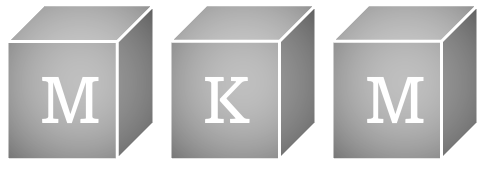
\includegraphics[width=0.4\textwidth]{../shared/Logos/MKM_logo.png}
    \end{figure}
    \vspace{1.5cm}
    {\Huge\bfseries\textcolor{mkmblue}{\doctitle}\par}
    \vspace{0.5cm}
    {\Large\textcolor{gray}{\docsubtitle}\par}
    \vspace{2cm}
    {\large MKM Research Labs\par}
    \vspace{0.5cm}
    {\large Version \docversion{} --- \docdate\par}
    \vspace{0.5cm}
    {\large \docauthor\par}
    \vspace{2cm}
    \textcolor{red}{\textbf{CONFIDENTIAL --- PROPRIETARY}}
    \end{center}
    \end{titlepage}
}

\newcommand{\mkmlegalpage}{%
    \clearpage
    \thispagestyle{empty}
    \begin{center}
    \large\textbf{Legal Notice}
    \vspace{1em}

    \textbf{PROPRIETARY AND CONFIDENTIAL}
    \end{center}

    \noindent This document, including all algorithms, models, methodology, formulas,
    calculations, and intellectual concepts contained herein, constitutes the exclusive
    intellectual property and confidential trade secrets of MKM Research Labs (``MKM'').

    \vspace{0.5em}
    \noindent Any usage, reproduction, distribution, modification, or disclosure of this
    document or any portion thereof, without the express prior written authorisation from
    MKM Research Labs is strictly prohibited and constitutes an infringement of intellectual
    property rights.

    \vspace{0.5em}
    \noindent The document is provided on an ``as is'' basis. MKM Research Labs makes no
    representations or warranties of any kind, express or implied, regarding its accuracy,
    reliability, or suitability for any particular purpose.

    \vspace{1em}
    \begin{center}
    All rights reserved. \copyright\ 2021--2026 MKM Research Labs.

    \vspace{0.5em}
    Governed by the laws of the United Kingdom.
    \end{center}
    \clearpage
}

\newcommand{\mkmhistorypage}[1]{%
    \section{Document History}
    \begin{table}[ht]
        \centering
        \begin{tabular}{l|l|l|l}
            \textbf{Date} & \textbf{Version} & \textbf{Description} & \textbf{Author} \\
            \hline
            #1
        \end{tabular}
        \label{tab:revision_history}
    \end{table}
    \clearpage
}

% ─── Bank validation protocol section commands ──────────────────────────────
% Use these to ensure every model doc has the required sections.
% They are just styled \section calls — content is provided by each doc.

\newcommand{\mkmexecsummary}{\section{Executive Summary}}
\newcommand{\mkmpurpose}{\section{Model Purpose and Scope}}
\newcommand{\mkmframework}{\section{Mathematical Framework}}
\newcommand{\mkminputs}{\section{Input Parameters and Calibration}}
\newcommand{\mkmimplementation}{\section{Implementation Details}}
\newcommand{\mkmsensitivity}{\section{Sensitivity Analysis}}
\newcommand{\mkmvalidation}{\section{Validation and Backtesting}}
\newcommand{\mkmtestresults}{\subsection{Automated Test Results}\input{test_results}}
\newcommand{\mkmlimitations}{\section{Model Limitations and Known Weaknesses}}

\newcommand{\mkmgovernance}{\section{Governance Validation Questions}
\noindent The following nine questions are mandated by Chapter~5 of the
\emph{Model Risk Governance for Vendors} handbook and must be explicitly
addressed for every model in the inventory. Response status is tracked in the
Model Governance Dashboard (MRC portal). \par\medskip}

\newcommand{\mkmvqitem}[3]{\subsection{Q#1 --- #2}
\noindent\textit{``#3''}\par\medskip\noindent}

\newcommand{\mkmchangelog}{\section{Change History}}
  (before \begin{document})
%
% Required commands before \input:
%   \newcommand{\doctitle}{...}
%   \newcommand{\docsubtitle}{...}
%   \newcommand{\docversion}{1.0}
%   \newcommand{\docdate}{13-February-2026}
%   \newcommand{\docauthor}{David K Kelly}

% ─── Packages ───────────────────────────────────────────────────────────────
\usepackage[utf8]{inputenc}
\usepackage{amsmath,amsfonts,amssymb}
\usepackage{listings}
\usepackage{color,xcolor}
\usepackage{graphicx}
\usepackage{hyperref}
\usepackage[toc,page]{appendix}
\usepackage{tabto}
\usepackage{float}
\usepackage{comment}
\usepackage[en-GB]{datetime2}
\usepackage{setspace}
\usepackage{subcaption}
\usepackage{booktabs}
\usepackage{longtable}
\usepackage{adjustbox}
\usepackage{enumitem}
\usepackage{fancyhdr}
\usepackage{lastpage}

% ─── Page geometry ──────────────────────────────────────────────────────────
\onehalfspacing
\usepackage{geometry}
\geometry{a4paper, total={170mm,247mm}, left=20mm, top=25mm, bottom=25mm}

% ─── Headers and footers ───────────────────────────────────────────────────
\pagestyle{fancy}
\fancyhf{}
\fancyhead[L]{\small\textcolor{gray}{MKM Research Labs}}
\fancyhead[R]{\small\textcolor{gray}{\doctitle{} --- v\docversion}}
\fancyfoot[C]{\small\textcolor{gray}{CONFIDENTIAL}}
\fancyfoot[R]{\small\textcolor{gray}{Page \thepage\ of \pageref{LastPage}}}
\renewcommand{\headrulewidth}{0.4pt}
\renewcommand{\footrulewidth}{0.4pt}

% ─── Colours ────────────────────────────────────────────────────────────────
\definecolor{mkmblue}{HTML}{1565C0}
\definecolor{codegreen}{rgb}{0,0.6,0}
\definecolor{codegray}{rgb}{0.5,0.5,0.5}
\definecolor{codepurple}{rgb}{0.58,0,0.82}
\definecolor{backcolour}{rgb}{0.95,0.95,0.92}

% ─── Hyperref setup ─────────────────────────────────────────────────────────
\hypersetup{
    colorlinks=true,
    linkcolor=mkmblue,
    citecolor=mkmblue,
    urlcolor=mkmblue
}

% ─── Code listings ──────────────────────────────────────────────────────────
\lstdefinestyle{mystyle}{
    backgroundcolor=\color{backcolour},
    commentstyle=\color{codegreen},
    keywordstyle=\color{magenta},
    numberstyle=\tiny\color{codegray},
    stringstyle=\color{codepurple},
    basicstyle=\ttfamily\footnotesize,
    breakatwhitespace=false,
    breaklines=true,
    captionpos=b,
    keepspaces=true,
    numbers=left,
    numbersep=5pt,
    showspaces=false,
    showstringspaces=false,
    showtabs=false,
    tabsize=2
}
\lstset{style=mystyle}

% ─── Section formatting ────────────────────────────────────────────────────
\setcounter{tocdepth}{3}
\setcounter{secnumdepth}{3}

% ─── Shared macros ──────────────────────────────────────────────────────────
\newcommand{\mkmtitlepage}{%
    \begin{titlepage}
    \begin{center}
    \vspace*{1cm}
    \begin{figure}[H]\centering
        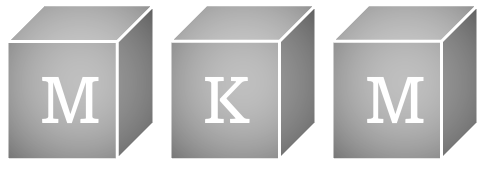
\includegraphics[width=0.4\textwidth]{../shared/Logos/MKM_logo.png}
    \end{figure}
    \vspace{1.5cm}
    {\Huge\bfseries\textcolor{mkmblue}{\doctitle}\par}
    \vspace{0.5cm}
    {\Large\textcolor{gray}{\docsubtitle}\par}
    \vspace{2cm}
    {\large MKM Research Labs\par}
    \vspace{0.5cm}
    {\large Version \docversion{} --- \docdate\par}
    \vspace{0.5cm}
    {\large \docauthor\par}
    \vspace{2cm}
    \textcolor{red}{\textbf{CONFIDENTIAL --- PROPRIETARY}}
    \end{center}
    \end{titlepage}
}

\newcommand{\mkmlegalpage}{%
    \clearpage
    \thispagestyle{empty}
    \begin{center}
    \large\textbf{Legal Notice}
    \vspace{1em}

    \textbf{PROPRIETARY AND CONFIDENTIAL}
    \end{center}

    \noindent This document, including all algorithms, models, methodology, formulas,
    calculations, and intellectual concepts contained herein, constitutes the exclusive
    intellectual property and confidential trade secrets of MKM Research Labs (``MKM'').

    \vspace{0.5em}
    \noindent Any usage, reproduction, distribution, modification, or disclosure of this
    document or any portion thereof, without the express prior written authorisation from
    MKM Research Labs is strictly prohibited and constitutes an infringement of intellectual
    property rights.

    \vspace{0.5em}
    \noindent The document is provided on an ``as is'' basis. MKM Research Labs makes no
    representations or warranties of any kind, express or implied, regarding its accuracy,
    reliability, or suitability for any particular purpose.

    \vspace{1em}
    \begin{center}
    All rights reserved. \copyright\ 2021--2026 MKM Research Labs.

    \vspace{0.5em}
    Governed by the laws of the United Kingdom.
    \end{center}
    \clearpage
}

\newcommand{\mkmhistorypage}[1]{%
    \section{Document History}
    \begin{table}[ht]
        \centering
        \begin{tabular}{l|l|l|l}
            \textbf{Date} & \textbf{Version} & \textbf{Description} & \textbf{Author} \\
            \hline
            #1
        \end{tabular}
        \label{tab:revision_history}
    \end{table}
    \clearpage
}

% ─── Bank validation protocol section commands ──────────────────────────────
% Use these to ensure every model doc has the required sections.
% They are just styled \section calls — content is provided by each doc.

\newcommand{\mkmexecsummary}{\section{Executive Summary}}
\newcommand{\mkmpurpose}{\section{Model Purpose and Scope}}
\newcommand{\mkmframework}{\section{Mathematical Framework}}
\newcommand{\mkminputs}{\section{Input Parameters and Calibration}}
\newcommand{\mkmimplementation}{\section{Implementation Details}}
\newcommand{\mkmsensitivity}{\section{Sensitivity Analysis}}
\newcommand{\mkmvalidation}{\section{Validation and Backtesting}}
\newcommand{\mkmtestresults}{\subsection{Automated Test Results}\input{test_results}}
\newcommand{\mkmlimitations}{\section{Model Limitations and Known Weaknesses}}

\newcommand{\mkmgovernance}{\section{Governance Validation Questions}
\noindent The following nine questions are mandated by Chapter~5 of the
\emph{Model Risk Governance for Vendors} handbook and must be explicitly
addressed for every model in the inventory. Response status is tracked in the
Model Governance Dashboard (MRC portal). \par\medskip}

\newcommand{\mkmvqitem}[3]{\subsection{Q#1 --- #2}
\noindent\textit{``#3''}\par\medskip\noindent}

\newcommand{\mkmchangelog}{\section{Change History}}
  (before \begin{document})
%
% Required commands before \input:
%   \newcommand{\doctitle}{...}
%   \newcommand{\docsubtitle}{...}
%   \newcommand{\docversion}{1.0}
%   \newcommand{\docdate}{13-February-2026}
%   \newcommand{\docauthor}{David K Kelly}

% ─── Packages ───────────────────────────────────────────────────────────────
\usepackage[utf8]{inputenc}
\usepackage{amsmath,amsfonts,amssymb}
\usepackage{listings}
\usepackage{color,xcolor}
\usepackage{graphicx}
\usepackage{hyperref}
\usepackage[toc,page]{appendix}
\usepackage{tabto}
\usepackage{float}
\usepackage{comment}
\usepackage[en-GB]{datetime2}
\usepackage{setspace}
\usepackage{subcaption}
\usepackage{booktabs}
\usepackage{longtable}
\usepackage{adjustbox}
\usepackage{enumitem}
\usepackage{fancyhdr}
\usepackage{lastpage}

% ─── Page geometry ──────────────────────────────────────────────────────────
\onehalfspacing
\usepackage{geometry}
\geometry{a4paper, total={170mm,247mm}, left=20mm, top=25mm, bottom=25mm}

% ─── Headers and footers ───────────────────────────────────────────────────
\pagestyle{fancy}
\fancyhf{}
\fancyhead[L]{\small\textcolor{gray}{MKM Research Labs}}
\fancyhead[R]{\small\textcolor{gray}{\doctitle{} --- v\docversion}}
\fancyfoot[C]{\small\textcolor{gray}{CONFIDENTIAL}}
\fancyfoot[R]{\small\textcolor{gray}{Page \thepage\ of \pageref{LastPage}}}
\renewcommand{\headrulewidth}{0.4pt}
\renewcommand{\footrulewidth}{0.4pt}

% ─── Colours ────────────────────────────────────────────────────────────────
\definecolor{mkmblue}{HTML}{1565C0}
\definecolor{codegreen}{rgb}{0,0.6,0}
\definecolor{codegray}{rgb}{0.5,0.5,0.5}
\definecolor{codepurple}{rgb}{0.58,0,0.82}
\definecolor{backcolour}{rgb}{0.95,0.95,0.92}

% ─── Hyperref setup ─────────────────────────────────────────────────────────
\hypersetup{
    colorlinks=true,
    linkcolor=mkmblue,
    citecolor=mkmblue,
    urlcolor=mkmblue
}

% ─── Code listings ──────────────────────────────────────────────────────────
\lstdefinestyle{mystyle}{
    backgroundcolor=\color{backcolour},
    commentstyle=\color{codegreen},
    keywordstyle=\color{magenta},
    numberstyle=\tiny\color{codegray},
    stringstyle=\color{codepurple},
    basicstyle=\ttfamily\footnotesize,
    breakatwhitespace=false,
    breaklines=true,
    captionpos=b,
    keepspaces=true,
    numbers=left,
    numbersep=5pt,
    showspaces=false,
    showstringspaces=false,
    showtabs=false,
    tabsize=2
}
\lstset{style=mystyle}

% ─── Section formatting ────────────────────────────────────────────────────
\setcounter{tocdepth}{3}
\setcounter{secnumdepth}{3}

% ─── Shared macros ──────────────────────────────────────────────────────────
\newcommand{\mkmtitlepage}{%
    \begin{titlepage}
    \begin{center}
    \vspace*{1cm}
    \begin{figure}[H]\centering
        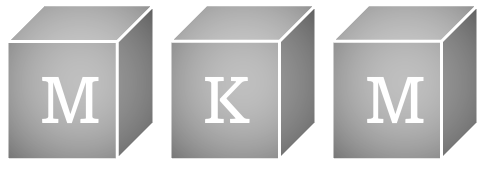
\includegraphics[width=0.4\textwidth]{../shared/Logos/MKM_logo.png}
    \end{figure}
    \vspace{1.5cm}
    {\Huge\bfseries\textcolor{mkmblue}{\doctitle}\par}
    \vspace{0.5cm}
    {\Large\textcolor{gray}{\docsubtitle}\par}
    \vspace{2cm}
    {\large MKM Research Labs\par}
    \vspace{0.5cm}
    {\large Version \docversion{} --- \docdate\par}
    \vspace{0.5cm}
    {\large \docauthor\par}
    \vspace{2cm}
    \textcolor{red}{\textbf{CONFIDENTIAL --- PROPRIETARY}}
    \end{center}
    \end{titlepage}
}

\newcommand{\mkmlegalpage}{%
    \clearpage
    \thispagestyle{empty}
    \begin{center}
    \large\textbf{Legal Notice}
    \vspace{1em}

    \textbf{PROPRIETARY AND CONFIDENTIAL}
    \end{center}

    \noindent This document, including all algorithms, models, methodology, formulas,
    calculations, and intellectual concepts contained herein, constitutes the exclusive
    intellectual property and confidential trade secrets of MKM Research Labs (``MKM'').

    \vspace{0.5em}
    \noindent Any usage, reproduction, distribution, modification, or disclosure of this
    document or any portion thereof, without the express prior written authorisation from
    MKM Research Labs is strictly prohibited and constitutes an infringement of intellectual
    property rights.

    \vspace{0.5em}
    \noindent The document is provided on an ``as is'' basis. MKM Research Labs makes no
    representations or warranties of any kind, express or implied, regarding its accuracy,
    reliability, or suitability for any particular purpose.

    \vspace{1em}
    \begin{center}
    All rights reserved. \copyright\ 2021--2026 MKM Research Labs.

    \vspace{0.5em}
    Governed by the laws of the United Kingdom.
    \end{center}
    \clearpage
}

\newcommand{\mkmhistorypage}[1]{%
    \section{Document History}
    \begin{table}[ht]
        \centering
        \begin{tabular}{l|l|l|l}
            \textbf{Date} & \textbf{Version} & \textbf{Description} & \textbf{Author} \\
            \hline
            #1
        \end{tabular}
        \label{tab:revision_history}
    \end{table}
    \clearpage
}

% ─── Bank validation protocol section commands ──────────────────────────────
% Use these to ensure every model doc has the required sections.
% They are just styled \section calls — content is provided by each doc.

\newcommand{\mkmexecsummary}{\section{Executive Summary}}
\newcommand{\mkmpurpose}{\section{Model Purpose and Scope}}
\newcommand{\mkmframework}{\section{Mathematical Framework}}
\newcommand{\mkminputs}{\section{Input Parameters and Calibration}}
\newcommand{\mkmimplementation}{\section{Implementation Details}}
\newcommand{\mkmsensitivity}{\section{Sensitivity Analysis}}
\newcommand{\mkmvalidation}{\section{Validation and Backtesting}}
\newcommand{\mkmtestresults}{\subsection{Automated Test Results}\input{test_results}}
\newcommand{\mkmlimitations}{\section{Model Limitations and Known Weaknesses}}

\newcommand{\mkmgovernance}{\section{Governance Validation Questions}
\noindent The following nine questions are mandated by Chapter~5 of the
\emph{Model Risk Governance for Vendors} handbook and must be explicitly
addressed for every model in the inventory. Response status is tracked in the
Model Governance Dashboard (MRC portal). \par\medskip}

\newcommand{\mkmvqitem}[3]{\subsection{Q#1 --- #2}
\noindent\textit{``#3''}\par\medskip\noindent}

\newcommand{\mkmchangelog}{\section{Change History}}

% T1 so the underscores in code identifiers print as underscores.
\usepackage[T1]{fontenc}
\usepackage{lmodern}
% Generated by tools.wolfram_oracle -- do not edit.
\newcommand{\bmGenerated}{2026-11-06}
\newcommand{\bmCodeCommit}{\texttt{ced02d123f9e}}
\newcommand{\bmCodeDirty}{}
\newcommand{\bmNumerics}{numpy 1.26.4, scipy 1.15.1, mpmath 1.4.1}
\newcommand{\bmWolfram}{15.0.0 for Mac OS X ARM (64-bit) (May 26, 2026)}
\newcommand{\bmWolframVia}{ via live kernel session (wolframclient)}
\newcommand{\bmWolframConfirms}{Wolfram, computing each independently, agrees with the reference to $2.3\times10^{-31}$.}
\newcommand{\bmChecks}{8}
\newcommand{\bmOutcome}{all pass}
\newcommand{\bmCodeErr}{$1.5\times10^{-14}$}
\newcommand{\bmHavErr}{$9.0\times10^{-10}$}
\newcommand{\bmTreeWrong}{0}
\newcommand{\bmTreeQueries}{1000}
\newcommand{\bmClaims}{13}
\newcommand{\bmClaimsMet}{13}
\newcommand{\bmClaimsFailed}{0}
\newcommand{\bmFigures}{27}

% The shared history table sets every column to its natural width; wrap the description.
\renewcommand{\mkmhistorypage}[1]{%
    \section{Document History}
    \begin{table}[ht]
        \centering
        \begin{tabular}{l|l|p{9cm}|l}
            \textbf{Date} & \textbf{Version} & \textbf{Description} & \textbf{Author} \\
            \hline
            #1
        \end{tabular}
    \end{table}
}

\begin{document}
% Long code paths and identifiers cannot hyphenate; let the spacing stretch instead.
\sloppy

\mkmtitlepage
\mkmlegalpage

\tableofcontents
\clearpage

% =========================================================================
\mkmexecsummary
% =========================================================================

This document benchmarks the Spatial Interpolation Model (MKM-SP-001): the module
\texttt{src/models/floodrisk/spatial.py}. It asks two questions. Does the code compute what
its model document (\texttt{spatial\_model\_v2.0.pdf}) says? And does what the document
says hold?

\paragraph{Version~0.1} tested the filed v1.0 of that document. The code computed its
distance and IDW exactly, but 10 of the document's 15 claims failed:
\begin{itemize}[leftmargin=*,nosep]
\item The spatial index treated a degree of latitude and of longitude as the same length.
  It named the wrong nearest gauge in 176 of 1{,}000 queries over the Thames basin.
\item The correlation was Euclidean degrees at 111\,km a degree, not the equation printed.
\item The coordinate path fixed the power and threshold.
\item Nothing returned the nearest gauge.
\item Nothing in the platform used the interpolation, the index or the correlation, and
  the tests, validation and kriging comparison the document cited did not exist.
\end{itemize}
The model was revised as v2.0:
\begin{itemize}[leftmargin=*,nosep]
\item the index on the unit sphere, with a lookup returning the nearest gauge and its
  distance;
\item the power and threshold taken from coordinates too;
\item its constants moved to config;
\item the document rewritten to say what the module computes, how accurate it is, and
  what uses it.
\end{itemize}
This version tests v2.0.

\paragraph{The code computes its documented equations.} The haversine agrees with a
50-digit implementation of v2.0's equations to \bmHavErr\,m. IDW from distances and from
coordinates, and the correlation, agree to \bmCodeErr. The index names the nearest gauge in
all \bmTreeQueries{} queries (Table~\ref{tab:bm-checks}). \bmWolframConfirms{}

\paragraph{The document's claims hold:} \bmClaimsMet{} of \bmClaims{}
(Table~\ref{tab:bm-claims}).
\begin{itemize}[leftmargin=*,nosep]
\item All \bmFigures{} figures in its tables reproduce from the code.
\item Its statements about the model are true: both interpolation paths take the power, and
  the correlation's conversion overstates east--west separation by 61\%. The sphere errs by
  the 0.32\% it states, and nothing in the platform calls what it says nothing calls.
\item Its statements about the evidence are true: the tests query the index, and there is
  no validation against observations and no kriging comparison.
\end{itemize}

\paragraph{Evidence.} \bmChecks{} checks, outcome: \bmOutcome{}
(Table~\ref{tab:bm-checks}).
\begin{itemize}[leftmargin=*,nosep]
\item Wolfram: \bmWolfram{}\bmWolframVia.
\item Code under test, at commit \bmCodeCommit{}\bmCodeDirty.
\item Numerics: \bmNumerics.
\item Generated \bmGenerated{} by \texttt{python -m tools.wolfram\_oracle sp001}.
\end{itemize}

% =========================================================================
\mkmpurpose
% =========================================================================

\subsection{What is benchmarked}
Every function in \texttt{spatial.py}:
\begin{itemize}[leftmargin=*,nosep]
\item \texttt{haversine\_distance};
\item the interpolation, from coordinates (\texttt{spatial\_interpolate\_wse}) and from
  distances (\texttt{idw\_interpolate\_from\_gauges});
\item the index (\texttt{build\_spatial\_index}, \texttt{nearest\_gauge});
\item the correlation matrix (\texttt{build\_correlation\_matrix});
\item the projection onto a segment and a polyline (\texttt{nearest\_point\_on\_segment},
  \texttt{nearest\_point\_on\_polyline}).
\end{itemize}
Its parameters are read from \texttt{config.models} (\texttt{\_spatial.py}).

\subsection{What is not}
\begin{itemize}[leftmargin=*,nosep]
\item Whether IDW or the correlation suits flood risk. v2.0 states that neither is
  validated or used (\S5, Q5).
\item The callers' own use of the distance and projection.
\end{itemize}
This is a benchmark of the implementation (validation question Q8), not independent
validation (Q9).

% =========================================================================
\mkmframework
% =========================================================================

The reference implements v2.0's equations directly from its text:
\begin{itemize}[leftmargin=*,nosep]
\item the haversine of Eq.~1, in its arctangent form, on a sphere of 6{,}371{,}000\,m;
\item the IDW of Eq.~2 with that distance and power $p$. The first gauge closer than the
  threshold (default 1\,m) returns its own value;
\item a gauge's water surface elevation as its depth plus its elevation (\S3.2);
\item the correlation of Eq.~3, on Euclidean degrees at 111\,km a degree;
\item the nearest gauge by Eq.~1 (\S3.3);
\item for the projection (\S3.5), the true nearest point on a segment drawn straight in
  latitude and longitude, found by minimising the haversine distance along it.
\end{itemize}

% =========================================================================
\section{Benchmark Method}
% =========================================================================

\paragraph{The cases.}
\begin{itemize}[leftmargin=*,nosep]
\item IDW: six gauge sets at seven powers from 0.5 to 4, including gauges inside the
  threshold and on it. The coordinate path: four gauges around a target on the Thames,
  with the target on a gauge, 0.5\,m from one, far off, and with a single gauge.
\item The correlation: five properties within 15\,km, $L=2$\,km, $\rho_0=0.6$.
\item The index: the case v1.0 got wrong, a gauge 0.010$^\circ$ north and one 0.012$^\circ$
  east of the target. Then 20 seeded random networks of 50 gauges over the Thames basin,
  queried at 50 random points each.
\item The projection: four segments (east--west, north--south, diagonal and 1\,km long).
  Points sit 10\,m to 200\,km from each midpoint, to the north, east and north-west.
  Nine points are projected onto a river-like polyline.
\end{itemize}

\paragraph{The printed tables.} Tables~2--5 were generated from the code. Each figure is
judged as the code's value printed to the places the table shows.

\paragraph{The statements.}
\begin{itemize}[leftmargin=*,nosep]
\item What the model accepts and returns is judged from the code.
\item What uses the model is judged by searching \texttt{src} and \texttt{scripts} for
  files that import the module and name each function.
\item Q4, Q5 and Q7 are judged by searching the repository: for tests that query the
  index, for any code that calls the interpolation, and for any mention of kriging.
\end{itemize}

\paragraph{Wolfram.} Wolfram works from each input's exact value, independently of the
reference:
\begin{itemize}[leftmargin=*,nosep]
\item the great-circle distance, as $R$ times the angle between the two points' unit
  vectors (not the haversine);
\item Eq.~2 at powers 2 and 5/2;
\item Eq.~3 from exact degrees;
\item the nearest point on the diagonal segment, where the squared chord along it is
  stationary (\texttt{FindRoot});
\item the true distance between six UK pairs under 100\,km, by \texttt{GeoDistance} on
  WGS84.
\end{itemize}

% =========================================================================
\mkmvalidation
% =========================================================================

% Generated by tools.wolfram_oracle -- do not edit.
\begin{table}[H]\centering\small
\caption{Benchmark checks}\label{tab:bm-checks}
\begin{adjustbox}{max width=\textwidth}
\begin{tabular}{p{96mm}p{16mm}rl}
\toprule
Check & Result & Limit & Outcome \\
\midrule
Eq.~1, the haversine: code against the reference, worst error (m) & $9.0\times10^{-10}$ & $1.0\times10^{-6}$ & pass \\
Eq.~2, IDW from distances, seven powers: worst relative error & $1.8\times10^{-16}$ & $1.0\times10^{-12}$ & pass \\
\S3.2, IDW from coordinates: WSE as depth plus elevation, Eq.~1's distance: worst relative error & $1.5\times10^{-14}$ & $1.0\times10^{-12}$ & pass \\
Eq.~3, the correlation at 111\,km a degree: worst relative error & $1.3\times10^{-15}$ & $1.0\times10^{-12}$ & pass \\
\S3.3, the index over 1000 queries: nearest gauges that differ from Eq.~1's & 0 & 0 & pass \\
\S3.3, the index's distance: worst relative error & $7.6\times10^{-13}$ & $1.0\times10^{-9}$ & pass \\
\S3.5, the polyline projection picks the reference's segment (9 points): segments that differ & 0 & 0 & pass \\
Wolfram agrees with the reference & $2.3\times10^{-31}$ & $1.0\times10^{-25}$ & pass \\
\bottomrule
\end{tabular}
\end{adjustbox}
\end{table}


\subsection{The model document's claims}
% Generated by tools.wolfram_oracle -- do not edit.
\begin{table}[H]\centering\small
\caption{The model document's claims, tested}\label{tab:bm-claims}
\begin{adjustbox}{max width=\textwidth}
\begin{tabular}{p{20mm}p{50mm}p{66mm}l}
\toprule
Claim & Stated & Benchmark finds & Outcome \\
\midrule
Table~1 & WSE by IDW power & 14 of 14 figures reproduced & met \\
Table~2 & WSE by distance of the nearest gauge & 7 of 7 figures reproduced & met \\
Table~2 & the gauge varied is the nearest & in 5 of 7 rows; at 5{,}000 and 10{,}000\,m the 2{,}000\,m gauge is nearer & \textbf{not met} \\
Table~3 & WSE by number of gauges & 5 of 5 figures reproduced & met \\
\S3.1, \S4.1 & the power and the 1\,m threshold are inputs & fixed at 2 and 1\,m where gauges are given by coordinates; inputs only where they are given by distance & \textbf{not met} \\
\S3.3 & the KDTree answers nearest-neighbour queries & it measures degrees of latitude and longitude alike, and names the wrong gauge in 176 of 1000 queries, up to 55\% farther; in the case built for it, the gauge 1112\,m away over one 831\,m away & \textbf{not met} \\
\S3.4, Eq.~3 & correlation decays with the distance $d$ of Eq.~1 & the code converts Euclidean degrees at 111\,km a degree; up to 98\% off Eq.~3 east--west & \textbf{not met} \\
\S4.2 & it returns the nearest gauge's distance and identity & no function returns a gauge & \textbf{not met} \\
\S5.1(2) & the haversine is sufficient below 100\,km (judged: within 0.5\% of WGS84) & worst -0.32\% & met \\
Q2 & the haversine is exact for the Earth's geometry & a sphere: -0.32\% from WGS84 & \textbf{not met} \\
\S5.2(3) & the flat-Earth projection errs beyond 50\,km & worst 0.0012\% within 50\,km; 0.019\% (39\,m) at 200\,km & met \\
\S1, \S2.1, Q1 & it maps gauge readings to properties by IDW, its exclusive use & nothing in \texttt{src} or \texttt{scripts} calls the interpolation, the index or the correlation; the haversine and projection serve the gauge, property, seismic code & \textbf{not met} \\
Q4 & unit tests verify KDTree correctness & no test queries the tree & \textbf{not met} \\
Q5 & outcomes are validated against held-out gauge readings & no code calls the interpolation to compare it with anything & \textbf{not met} \\
Q7 & IDW is compared against kriging and nearest-neighbour baselines & kriging appears nowhere in the repository & \textbf{not met} \\
\bottomrule
\end{tabular}
\end{adjustbox}
\end{table}


% =========================================================================
\mkmlimitations
% =========================================================================

\begin{enumerate}[leftmargin=*]
\item \textbf{Benchmark, not validation.} The code is shown to compute its documented
  equations, and the document to describe it. Whether IDW represents a flood surface is
  not tested. v2.0 says so, and nothing in the repository tests it.
\item \textbf{Searches are of this repository.} ``Nothing calls it'' means nothing in
  PhysicalRisk at the commit above.
\item \textbf{The index is judged on random networks} over the Thames basin. It is exact
  by construction (\S3.3), so the networks test the code, not the method.
\end{enumerate}

\mkmhistorypage{06-Nov-2026 & 0.1 & First issue: tests the filed v1.0; 10 of its 15 claims fail (not filed) & David K Kelly \\
06-Nov-2026 & 0.2 & Tests v2.0, the revised model & David K Kelly \\}

\end{document}
